\documentclass[../notes.tex]{subfiles}

\pagestyle{main}
\renewcommand{\chaptermark}[1]{\markboth{\chaptername\ \thechapter\ (#1)}{}}
\setcounter{chapter}{5}

\begin{document}




\chapter{Molecular Dynamics}
\section{Chemical Exchange and DOSY}
\begin{itemize}
    \item \marginnote{3/11:}Lecture outline.
    \begin{itemize}
        \item Chemical exchange.
        \item PFGs and DOSY.
        \item PSet 4.
        \item Final project.
    \end{itemize}
    \item PSet 4: ROESY and NOESY for Aflatoxin B1.
    \begin{itemize}
        \item Understand why there are three peaks in the ROESY.
        \item What do they mean? Where do they come from? Should there be others?
        \item This is a fairly simple, \SI{400}{\milli\second} ROESY.
        \item NOESY does not look as nice.
        \begin{itemize}
            \item But looks better after phase and baseline spectrum.
            \item You can also adjust the density/level of contours. This makes peaks more defined.
        \end{itemize}
    \end{itemize}
    \item Make sure to properly phase and baseline 2D spectra, too!
    \begin{itemize}
        \item How do you do this??
        \item There are equivalents in MNova.
        \item Capture a place in the spectrum in Interactive Phase Correction, look at the columns.
        \item Zero-order phase correction at the pivot, first-order phase correction at the sides.
        \item \emph{Automatic} phase and baseline correction can be good, too.
    \end{itemize}
    \item Chemical exchange and NMR timescales in \emph{N},\emph{N}-dimethylacetamide (DMA).
    \begin{itemize}
        \item Methyls are in two different chemical environments at room temperature, but they merge into one peaks at higher temperatures. It's like a high-temperature equivalent of cyclohexane ring flipping at low temperatures!
        \item Proton peaks get closer together and broader at higher temperatures, before coalescing. You have a point at which the exchange rate (rotation around the bond) is basically equal to the chemical shift difference (in hertz).
        \item The difference between the two signals in hertz tells you the exchange rate!
        \item Glenn Facey (NMR tech at University of Ottawa) has some really good examples in his blog.
        \item Two broad peaks may be different compounds, or \textbf{rotamers}; the typical test is heating up!
        \item Coalescence happens for carbon at a higher temperature than for protons! Sometimes, your signal just goes away/disappears into the background.
    \end{itemize}
    \item \textbf{Rotamer}: A molecule that has two forms differentiated by rotation about a chemical bond.
    \item If the populations are equal, the final average will be equidistant between the two; if the populations are unequal, the final average will be weighted.
    \item Examples of chemical exchange.
    \begin{itemize}
        \item Often tertiary amides (restricted bond rotation).
        \item Ring flipping.
        \item Tautomerization (e.g., $6\pi$ electrocyclization in cyclohepta-1,3,5-trienes).
        \item Center inversion (i.e., nitrogens becoming chiral at low temperatures).
        \item Rearrangement reactions.
        \item \textbf{Fluxionality}.
    \end{itemize}
    \item Protonated tertiary nitrogens (with TFA vapor) may be useful for rotamers??
    \item \textbf{Pulsed field gradient}: Allow for the precies introduction of a linear field gradient across the sample. \emph{Also known as} \textbf{PFG}.
    \begin{itemize}
        \item Using molecular tumbling to figure out how big molecules are.
        \item Your proton gets super spread out, e.g., over \SI{200}{\partspermillion}.
        \item Instead of a Fourier transform, you apply a \textbf{Laplace transform} (or \textbf{Bayesian processing}) to figure out diffusion time and correlate that to molecular weight.
        \item To correlate diffusion coefficient to weight, you have to understand the viscosity of the solvent, temperature, fluid effects, etc.
        \item May need to convert data from 2D to a 1D stack, rephase, and rebaseline.
        \item You can make MNova do a Bayesian transform.
        \item Mixes of multiple molecules will give you two different diffusion coefficients!
        \begin{itemize}
            \item This could help with identifying if my unknown sample in lab is multi-component or just one molecule!
            \item I could also TLC/chromatograph the sample.
        \end{itemize}
    \end{itemize}
    \item PSet 4 will be assigned today, and we'll have a week to do it.
    \item The final project.
    \begin{itemize}
        \item Propose a particular chemical synthesis that we're interested in, ask what I'd like to see come out at the other end, and how could I use the NMR experiments in class to distinguish between products?
    \end{itemize}
    \item Chemical shift prediction (\ce{{}^13C}, \ce{{}^15N} can guide our thought, but it shouldn't determine our assignments).
    \begin{itemize}
        \item Aflotoxin's precisely-defined stereochemistry across the bridged ring will come in.
    \end{itemize}
    \item PSet 3.
    \begin{itemize}
        \item The carbons I couldn't identify are all exchange-broadened, in the \SIrange{150}{160}{\partspermillion}.
        \item Should have HMBCs to nearby protons.
    \end{itemize}
\end{itemize}



\section{Suppressing Unwanted Signals}
\begin{itemize}
    \item \marginnote{3/13:}DOSY?
    \begin{itemize}
        \item Can be run in automation with Walt's approximate parameters on 500 and 600.
        \item If I want to learn how to optimize the parameters for DOSY, ask Bridget (the DOSY expert) to schedule a training time. We'll optimize it on 501 (manual), and then I can run the optimized parameters on any automation system.
        \item DOSY is not good at separating peaks "vertically," i.e., different compounds that have something with the same chemical shift. Though there are ways around this.
        \item Yuzhe and Eddy also are pretty good at DOSY, per Yuzhe.
    \end{itemize}
    \item Lecture outline.
    \begin{itemize}
        \item Filtering experiments.
        \item Composite experiments.
    \end{itemize}
    \item Everything that's been talked about in this class can be done in an automated fashion, as long as we know which parameters to dial in. Everythign that's been talked about can also be done manually, again as long as we know what to dial in.
    \item More on DOSY.
    \begin{figure}[h!]
        \centering
        \begin{subfigure}[b]{0.3\linewidth}
            \centering
            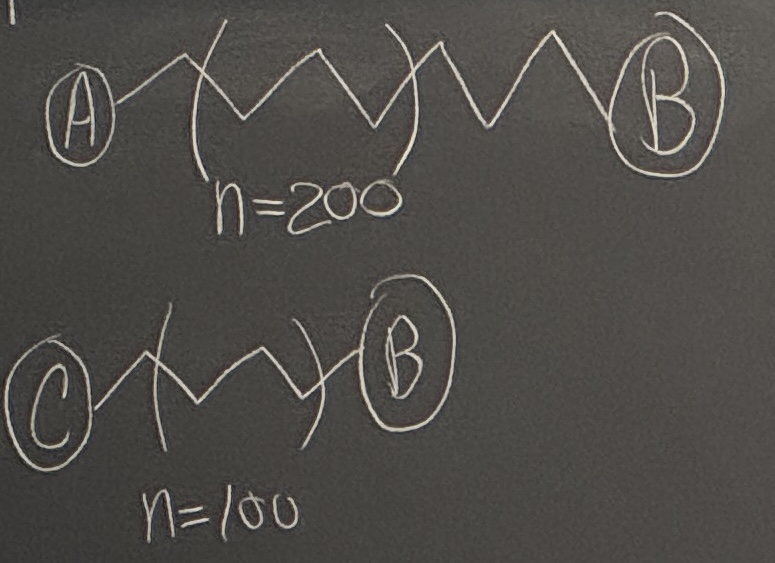
\includegraphics[width=0.8\linewidth]{DOSYa.JPG}
            \caption{Species in mixture.}
            \label{fig:DOSYa}
        \end{subfigure}
        \begin{subfigure}[b]{0.3\linewidth}
            \centering
            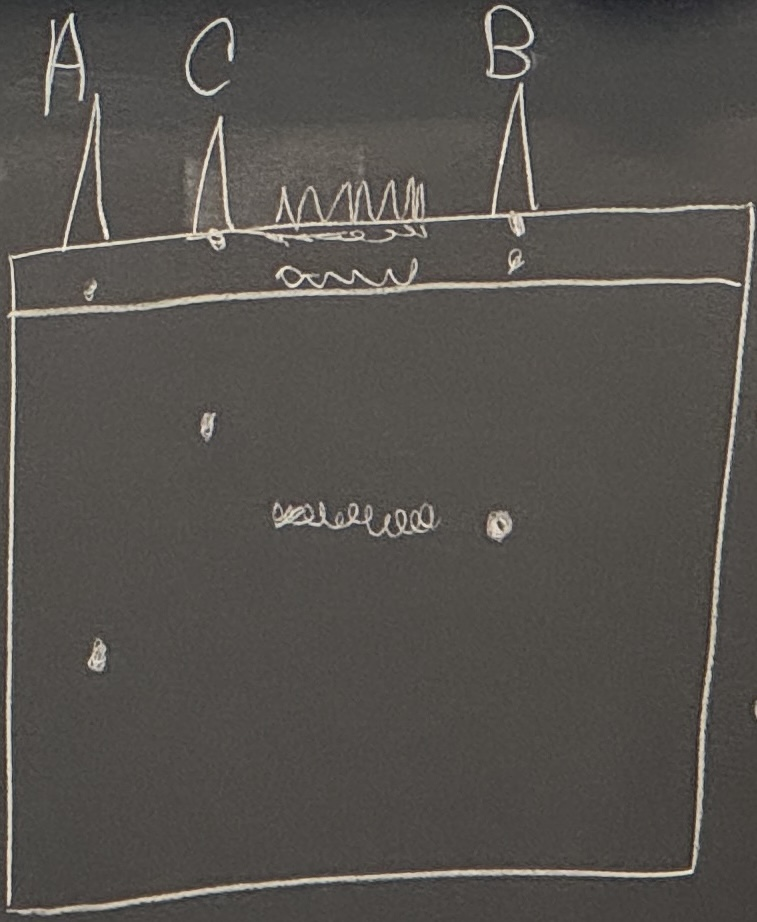
\includegraphics[width=0.8\linewidth]{DOSYb.JPG}
            \caption{DOSY spectrum.}
            \label{fig:DOSYb}
        \end{subfigure}
        \begin{subfigure}[b]{0.3\linewidth}
            \centering
            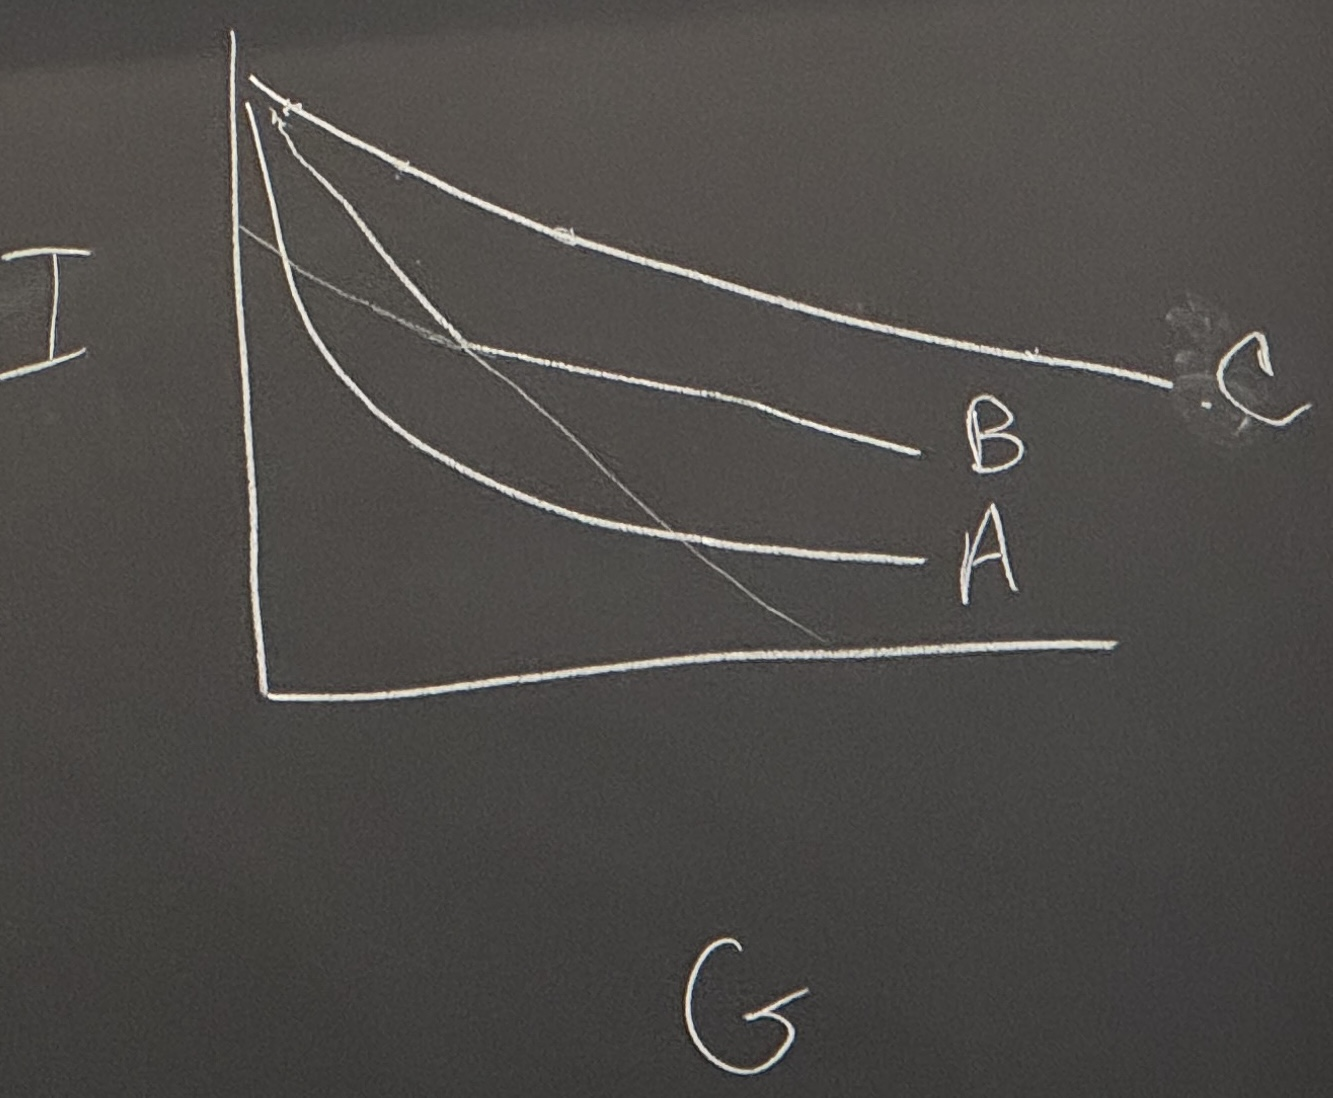
\includegraphics[width=0.8\linewidth]{DOSYc.JPG}
            \caption{Gradient plot.}
            \label{fig:DOSYc}
        \end{subfigure}
        \caption{DOSY with overlapping peaks.}
        \label{fig:DOSY}
    \end{figure}
    \begin{itemize}
        \item Imagine you have two different polymer species (100 repeat units, 200 repeat units; A-B end groups vs. C-B end groups).
        \item All chemical shift is summed along the chemical shift axis (\ce{{}^1H} NMR spectrum of A-B plus C-B).
        \item Signals for the middle stuff goes to a weighted average, B goes to weighted average, C is up top, and A is at bottom.
        \item Can also anaylze the data as a plot of integrated intensity vs. gradient strength, which is also the way the experiment is actually done.
        \begin{itemize}
            \item Bigger molecule's intensity decays more rapidly at higher gradients.
            \item For \ce{B}, one part maps with \ce{A} and one with \ce{C}, so you can do careful analysis and better estimate what the middle signals are telling you.
            \item You need to do careful analysis in MNova and learn from Bridget.
        \end{itemize}
        \item To reiterate: There's a sense that DOSY is \emph{great} for MW measurement. But in reality, DOSY is just \emph{good} for \emph{estimating} molecular weight; really getting accuracy requires mass spec.
    \end{itemize}
    \item Spin echo.
    \begin{itemize}
        \item Very good for NMR filtering and separating signals from each other.
        \item Let all the noise from the receiver pulse die away, then do a \ang{180} pulse and get your signal cleanly.
        \item 1-2 Nobel prizes in the 1950s for developing this idea.
    \end{itemize}
    \item Filtering experiments: CPMG.
    \begin{itemize}
        \item Instead of just one spin echo, you can use two or more.
        \item The 600's probe has a big carbon background, but using a double echo can filter out the broad part.
        \item We can see the background in PSet 4, experiment 12.
        \begin{itemize}
            \item Related to 1012, and subtraction.
            \item Double echo carbon and simple carbon.
        \end{itemize}
    \end{itemize}
    \item Presaturation.
    \begin{itemize}
        \item Sometimes, you can saturate the water signal in \ce{MeOD}, because if exchange is fast enough, this will saturate the \ce{MeOH} protons, too, when exchanged.
    \end{itemize}
    \item Excitation sculpting.
    \begin{itemize}
        \item zgesgp on the NMR systems.
        \item If it's really important to your advisor (e.g., Mo) to suppress the \ce{CDCl3} residual signal when you publish the spectrum, do something very gentle like this.
    \end{itemize}
    \item "Wet" experiment.
    \begin{itemize}
        \item Here, you can look at solutes in LC-NMR.
        \item Pretty good at preserving the signals overlapped with the solvent peak.
    \end{itemize}
    \item VNC Viewer allows you to remote into the spectrometers.
    \item HSQC correlates protons to carbons, but wouldn't it be great if we could attach that proton to other protons, too? This is the HSQC-TOCSY.
    \begin{itemize}
        \item This connects a carbon to its proton(s), and also some nearby protons.
        \item This helps with proton chemical shift overlaps, which a real TOCSY can't help with much.
        \item This vs. HMBC?
        \begin{itemize}
            \item Can give different peaks from HMBC.
            \item In a perfect world, where all coupling constants are big enough to measure, they give the same data.
            \item Doesn't run much faster than an HMBC.
        \end{itemize}
        \item You can also do HSQC-NOESY's, etc.
        \item How do you run these in the DCIF??
    \end{itemize}
    \item HSQC, no decoupling.
    \begin{itemize}
        \item Everything is centered on the HSQC peaks and split by the ${}^1J_{\ce{CH}}$ coupling constant.
    \end{itemize}
    \item HSQC-DOSY.
    \begin{itemize}
        \item Overlapping proton chemical shift, but non-overlapping carbon chemical shift.
    \end{itemize}
\end{itemize}




\end{document}